%
% PROJECT: <ETD> Electronic Thesis and Dissertation Initiative
%   TITLE: LaTeX report template for ETDs in LaTeX
%  AUTHOR: Kayla Straub, kstraub@vt.edu
% SAVE AS: Straub_KM_T_2016.tex
% REVISED: February 17, 2016
% 


\documentclass[12pt]{report}

\usepackage{times}
\usepackage{times}
\usepackage{graphicx}
\usepackage{amsmath}
\usepackage{amsthm, amssymb}
\usepackage{enumerate}
\usepackage{fullpage}
\usepackage{hyperref}
\usepackage{soul}
\usepackage{xcolor}
\usepackage{comment}
\usepackage{listings}
\usepackage{color} %red, green, blue, yellow, cyan, magenta, black, white
\definecolor{mygreen}{RGB}{28,172,0} % color values Red, Green, Blue
\definecolor{mylilas}{RGB}{170,55,241}
\usepackage{fancybox}
\usepackage{framed}
\usepackage{mathrsfs}
\usepackage{url}
\usepackage{paralist}
\usepackage{booktabs}
\usepackage{floatrow}
\floatsetup[table]{capposition=top}
\usepackage[font=small,labelfont=bf]{caption}
\usepackage{fancyhdr} % Used for header
\usepackage[headsep=0.5cm,headheight=0.5cm]{geometry}


\hypersetup{breaklinks=true}
\urlstyle{same}


\graphicspath{{Pictures/}}


\setlength{\textwidth}{6.5in}
\setlength{\textheight}{8.5in}
\setlength{\evensidemargin}{0in}
\setlength{\oddsidemargin}{0in}
\setlength{\topmargin}{0in}

\setlength{\parindent}{0pt}
\setlength{\parskip}{0.1in}

% Uncomment for double-spaced document.
\renewcommand{\baselinestretch}{2}

\usepackage{epsf}

\begin{document}

\thispagestyle{empty}
\pagenumbering{roman}
\begin{center}

% TITLE
{\Large 
Data Mining Academic Emails to Model Employee Behaviors and Analyze Organizational Structure
}

\vfill

Kayla M. Straub

\vfill

Thesis submitted to the Faculty of the \\
Virginia Polytechnic Institute and State University \\
in partial fulfillment of the requirements for the degree of

\vfill

Master of Science \\
in \\
Electrical Engineering
\vfill

Robert W. McGwier, Chair \\
Aloysius A. Beex\\
Michael M. Buehrer\\
Bert Huang

\vfill

March 25, 2016 \\
Blacksburg, Virginia

\vfill

Keywords: 
\\
Copyright 2016, Kayla M. Straub

\end{center}

\pagebreak

\thispagestyle{empty}
\begin{center}

{\large Data Mining Academic Emails to Model Employee Behaviors and Analyze Organizational Structure}

\vfill

Kayla M. Straub

\vfill

(ABSTRACT)

\vfill

\end{center}

[This is just the paper abstract - I plan to rewrite this near the end].
Email correspondence has become the predominant method of communication for businesses.
If not for the inherent privacy concerns, this electronically searchable data could be used to better understand how employees interact. 
For example, after the Enron dataset was made available, researchers were able to provide great insight into employee behaviors based on the available data despite the many challenges with that dataset.  
The work in this paper demonstrates the application of a suite of methods to an appropriately anonymized email dataset created from volunteers' email metadata.  
This new dataset, from an internal email server, is first used to validate machine learning and feature extraction algorithms and then to generate insight into the interactions within the center.  
Based solely on email metadata, a random forest approach modeled behavior patterns and accurately classified employees by job title.  
The algorithm performed very well not only on participants in the study but also on other members of the center who were connected to participants through email. 
Furthermore, the data revealed relationships not present in the formal operating structure. 
The result is a much fuller understanding of the center's internal structure than can be found in the official organization chart.


\vfill

% GRANT INFORMATION


\pagebreak

% Dedication and Acknowledgments are both optional
\chapter*{Dedication}
\chapter*{Acknowledgments}

\tableofcontents
\pagebreak

\listoffigures
\pagebreak

\listoftables
\pagebreak

\pagenumbering{arabic}
\pagestyle{myheadings}

\chapter{Introduction} \label{Introduction}
\section{Motivation}
A reorganization of a business can be very costly and has great effects once implemented, either for better or for worse.
While this official hierarchy is important, there is an equally important organic organization of any business, which may or may not be reflected in the official organization chart.
Understanding this unofficial structure is important, but due to its informal nature, it can be difficult to determine.
One massive source of electronically searchable information that could be used to better understand this hidden structure is the business's emails.
However, privacy concerns inhibit most research thrusts into email analysis.  

If access was given to email metadata, there could be several potential applications to this information beyond gaining a better understanding of the organizational structure.  It could be possible ot identify people of influence or potential leaders.  By recognizing changing behavior, potential insider treats could be identified.

\section{Problem Overview}
The study presented in this paper collected an appropriately anonymized email metadata dataset to demonstrate to what extent this metadata can be used to determine an organic organizational chart.
Furthermore, this research measured how well this organic organizational chart matches the official organizational chart.
The study utilized email metadata from 37 voluntary participants.
This metadata is used not only to analyze the voluntary participants, but also to what extent the non-participant members of the organization can be characterized.
\section{Approach}
The 98 features used in this study can be grouped into two common areas in email analytics: traffic-based and social-based.
Using random forests, these features are used to predict each employee's job title.
The ability to accurately determine job title using as few as three features is demonstrated.
Finally, a comparison between relationships displayed in the data with the formal organizational chart is presented.  
\section{Contributions}
The contributions outlined in this thesis are broad.  First, a new, fully anonymized dataset was developed from raw emails from an academic research environment.  This dataset, unlike others before it, has accurate job title labels.  Furthermore, a unique combination of features were calculated from this data.  Many had been used in email analysis before, but some are new and specific to this data.  In general, the problem of job title classification has not been extensively studied.  However, the results in this thesis surpass the results of previous research.
\section{Outline}
This paper continues by discussing the related works in Section~\ref{PriorWork}.  
Section~\ref{Data} describes the process of data collection and some statistics of the dataset and the features extracted from the data.
The methods investigated using these features are covered in Section~\ref{Algorithm}.
The results of the analysis are presented in Section~\ref{Performance}.
 Section~\ref{FutureWork} presents opportunities for future work, and Section~\ref{Conclusions} concludes the thesis.


\chapter{Prior Work} \label{PriorWork}
\section{Background}
Email is a pervasive medium for communication in modern society\textemdash{}particularly in the workplace.
In 2015, there were over 2.6 billion email users~\cite{radicati_emails_2015}.
It is projected that by the end of 2019, over one third of the global population will be using email.
In fact, the average business email user sends and receives a total of 112 emails per day.
Corporate email alone accounts for 54.7\% of worldwide email traffic.
Retention of large email archives has become common practice with decreasing memory size and cost~\cite{fisher_revisiting_2006}.
Out of 600 employees at a high-tech company, the average employee had 28,660 emails stored in 133 folders which is a significant increase over the past ten years.
This is a considerable amount of untapped information that could be leveraged to characterize employee roles within an organization.
\section{Commonly Used Datasets}
Since the Enron email dataset was released in 2004 \cite{klimt_introducing_2004}, it has been extensively researched on topics including spam classification~\cite{gaber_e-mail_2016}, \cite{shams_classifying_2013}; email categorization \cite{he_novel_2014}, \cite{keila_structure_2005}; and recipient prediction \cite{sofershtein_predicting_2015}, \cite{hu_towards_2012}.
However, there are known flaws and discrepancies with even the most recent versions of this dataset\textemdash{}ranging from misspelled email addresses~\cite{nordbo_data_2014} to duplicate email addresses~\cite{waterman_big_2014}, and misfiled emails~\cite{namata_inferring_2006}.
In one of the most popular forms of the dataset~\cite{shetty_enron_2004}, the database includes 253,735 emails sent as ``CC'' and  253,713 emails sent as ``BCC''.
Further inspection reveals that emails sent as one type or the other were almost always mistakenly recorded as both.  In addition to all of these issues, no comprehensive or accurate list of job title labels is available.
\section{Prior Analysis}
The existing literature on analyzing social email behavior is mainly divided into two categories: traffic-based and social-based~\cite{tang_email_2013}.
Traffic-based methods calculate statistics based only on email patterns.
Social-based methods represent the email communications as a social graph and then extract information from this model using graph-based algorithms.

Using features extracted from email metadata,~\cite{yelupula_social_2008} was able to cluster levels of management at Enron.
In addition to email traffic statistics, using features such as the presence of different email attachment types and the length of emails was shown to successfully categorize email behavior in~\cite{martin_analyzing_2005}.

Relational ties can be modeled as a graph network where nodes represent people and edges represent email interactions.
This is a useful model because many statistics can be calculated from the layout of a social graph~\cite{wasserman_social_1994}.
A common metric that has been shown to indicate importance in a social graph is betweenness centrality, which comes in several different flavors first developed by~\cite{freeman_set_1977}.
Betweenness centrality is a measure of how many shortest paths in a graph travel over each node.
A node with high betweenness centrality in a social graph has been shown to represent a high degree of influence on other nodes.
As shown in~\cite{tyler_email_2003}, a betweenness centrality algorithm can be used to determine community structures within an organization.
Other successful metrics were used in~\cite{wilson_discovery_2009}, which detected the most important email users within a corporate network without using betweenness as a feature.
The features used in that study were: degree, the number of edges connected to a node; density, the ratio of actual edges to the number of possible edges; and proximity prestige, the ratio of nodes that can reach a node $i$ to the average distance from those nodes to $i$.

Instead of considering only traffic-based or social-based analytics, these can be be used jointly.
An example of this approach~\cite{rowe_automated_2007}, which combined features such as number of emails, response time, cliques, and degree centrality into a ``Social Score'', was used to rank Enron employees.  

\chapter{Email Dataset and Feature Extraction} \label{Data}

Over the past decade, the Enron dataset has been widely used to study email behaviors because it is one of the only datasets available comprised of real-world corporate emails.
A list of ground truth job titles was compiled by~\cite{shetty_status_2004}.  However, there are known issues with these labels.
Due to difficulties with the Enron dataset, as described in Section~\ref{PriorWork}, this study uses a new dataset generated from volunteers in one of the university's centers.

\section{Data Collection}
Due to the inherent privacy concerns, researchers worked with the Internal Review Board (IRB) to approve a dataset which maintains participants' privacy.
This dataset is meant to be representative of metadata which any company could use without violating the privacy of their employees.
Special care was taken to protect the privacy of those involved in the study.
During the collection process, all subject and body text was hashed, and all email metadata was stored in a MySQL database using scripts without any researchers observing any email text.
Furthermore, any identifying information has been omitted from this publication.

The center's email server offers the ability to both digitally sign and encrypt emails.  Sending an email with either or both of these options appears as a special type of attachment in the raw email file.  Therefore, during the data collection process, information about if an email was signed or encrypted was recorded.  This process was part of the comprehensive parser script developed for extracting information from each email.

The following is the metadata parsed from each email:
\begin{compactitem}
\item Destination and source email address
\item Email time stamp
\item Subject prefix (e.g., Re:, Fwd:)
\item Hash of subject after removing prefix
\item Hash of body text
\item Length of subject in characters
\item Length of body text in characters
\item Number of attachments
\begin{compactitem}
\item Indicator if email was digitally signed
\item Indicator if email was encryped
\end{compactitem}
\end{compactitem}


\section{Dataset Description and Statistics}
Table~\ref{tab:db_stats} compares statistics between this internal dataset and the Enron corpus.
This internal database is more modern, contains more emails, and covers a longer time period.
However, it is comprised of fewer people than the Enron dataset.

\begin{table}[t]
\centering
\caption{A comparison between the internal dataset and the Enron email corpus.}
\label{tab:db_stats}
\resizebox{0.6\textwidth}{!}{%
\begin{tabular}{@{}lrr@{}}
\toprule
                   & Center          & Enron         \\ \midrule
Time               & 11/2012-11/2015 & 1/2000-9/2002 \\
Distinct Email Addresses & 32,118          & 75,406        \\
Participants       & 37              & 249           \\
Distinct Emails    & 585,096         & 252,759       \\ \bottomrule
\end{tabular}
}
\end{table}

The center divides its employees into six main areas: directors, graduate students, operations, outreach, project management (PM), and research. 
A chart showing the distribution of classes is shown below in Figure \ref{fig:class_breakdown}
\begin{figure}[t]
    \centering
        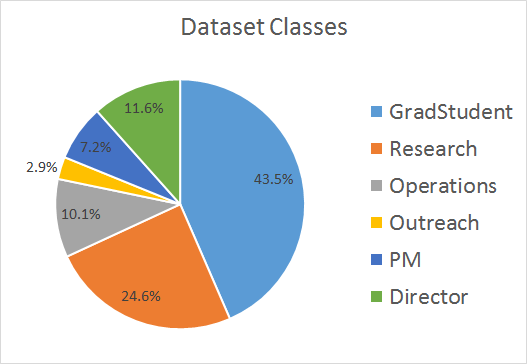
\includegraphics[width=\columnwidth,trim={1mm 8mm 1mm 2mm},clip]{class_breakdown}
        \caption[Dataset class distribution pie chart]{Pie chart showing the distribution of classes in the dataset.  Note that the classes are far from being uniformly distributed.}
        \label{fig:class_breakdown}
\end{figure}


While the study includes only 37 volunteers, the email metadata from these volunteers identified 32 additional employees of the center.
These additional employees were included in the study when ground truth for their job was available and when they were identified in at least 100 email metadata records.
This provides 69 total employees in the study.

\section{Features}
The study includes 111 features that were extracted from the email data: 80 traffic-based and 31 social-based.
The traffic-based features are those calculated purely from the collected email metadata.
The social features, on the other hand, first model the email patterns in a graphical network and then calculate statistics from this model.
In the following sections, all features from each of the two categories are described. 

\subsection{Traffic-Based Features}
\subsubsection{Email Counts and Email Types}
The simplest traffic-based features involve counting how many and what kinds of emails each participant sends and receives.
First, the total number of emails, total sent, and total received give a measure of how active an email user is on average.
These features can also indicate the direction tendencies of an employee's communication. 
Do they send more emails than they receive, or vice versa?  All of the traffic-based features detailed below consider direction.
Specifically, each metric is calculated three times: considering only sent emails, only received emails, and both sent and received emails.

Some traffic-based features focus on the different types of emails.
Two examples of these types of features are the number of emails sent directly to each employee and the number of emails where they were carbon copied on the email.
The opposite direction of this was inspected as well, that is, the number of emails the employees sent directly to others and the number of carbon copies sent out.
The average number of recipients on emails sent and received for each participant were also calculated.
Similarly, the number of emails sent and received as replies or forwards were used.
These measures give a sense of how the employee communicates with others in the organization and their connectedness.

Several features were calculated from just the subset of emails that were digitally signed.  These features were the total number of emails sent and received, number of unique email addresses, and the number of unique subjects.
These same metrics were also calculated for encrypted emails.

\subsubsection{Metadata Statistics}
The metadata of the emails contains extremely useful information.  This includes the email addresses involved, time stamp, the subject and body hashes and character counts, and the presence of any attachments.
From the time stamp, the time of day for each email was available.
The total number of emails with timestamps after hours were used as a metric.
For this purpose, after hours was defined as between 6pm and 7am EST on weekdays or anytime on weekends.
The timestamps were also used to calcualate the average number of emails per day for each employee.
The mean and variance of the number of characters in the subject and body were calculated.
The total number of attachments sent and received were computed as well as the average number of attachments per email.

Some of the most interesting information came from email addresses and subject hashes of the emails.
The number of unique email address connections, both sent and received, was used as a feature.
By counting the number of identical hashed subjects, it was determined how many unique subjects were both sent and received from each employee.
The motivation behind these features is that employees with particular job titles may be more likely to be associated with long email chains, which would have the same subject.
It was hypothesized that staff members had more external communications than graduate students.
To test this, the number of emails sent and received from within the center and the university were calculated.
Email addresses with a Virginia Tech domain were considered to be affiliated with the university.
Email addresses with accounts on the internal mail server were labeled to be within the center.
Note that all employee email addresses of the center have a Virginia Tech domain, and are therefore also considered to be part of the university.


Most of the features described above involved raw email counts.
However, this could skew data by giving more importance to employees who have been associated with the center longer.
In order to normalize these values, corresponding percentage values were also fed into the learning algorithm.
Examples include the percentage of  sent emails that were sent after hours and the percentage of received emails with unique subjects out of all received emails.



\subsubsection{Most Useful Traffic-Based Features}
The best traffic-based feature for predicting employee status was the number of unique subjects received.
The metric used to evaluate features is information gain.  This was used because it is integral to the machine learning algorithm described in Section~\ref{Algorithm}; details on the feature ranking analysis are provided in that section.
This number of unique subjects received represents how many distinct conversations involve each individual.
It is intuitive that people who are involved in more conversations hold a higher position in an organization because their input is requested more often.
A histogram showing the different values for this metric over the different job classes is shown in Figure~\ref{fig:traffic_ex_hist}.
It is clear from the figure that GradStudents participated in far fewer email conversations than any other group.
Researchers generated more emails on average, but fewer than the Program Managers.
The directors of the center participate in the most email conversations. 
\begin{figure}[t]
    \centering
        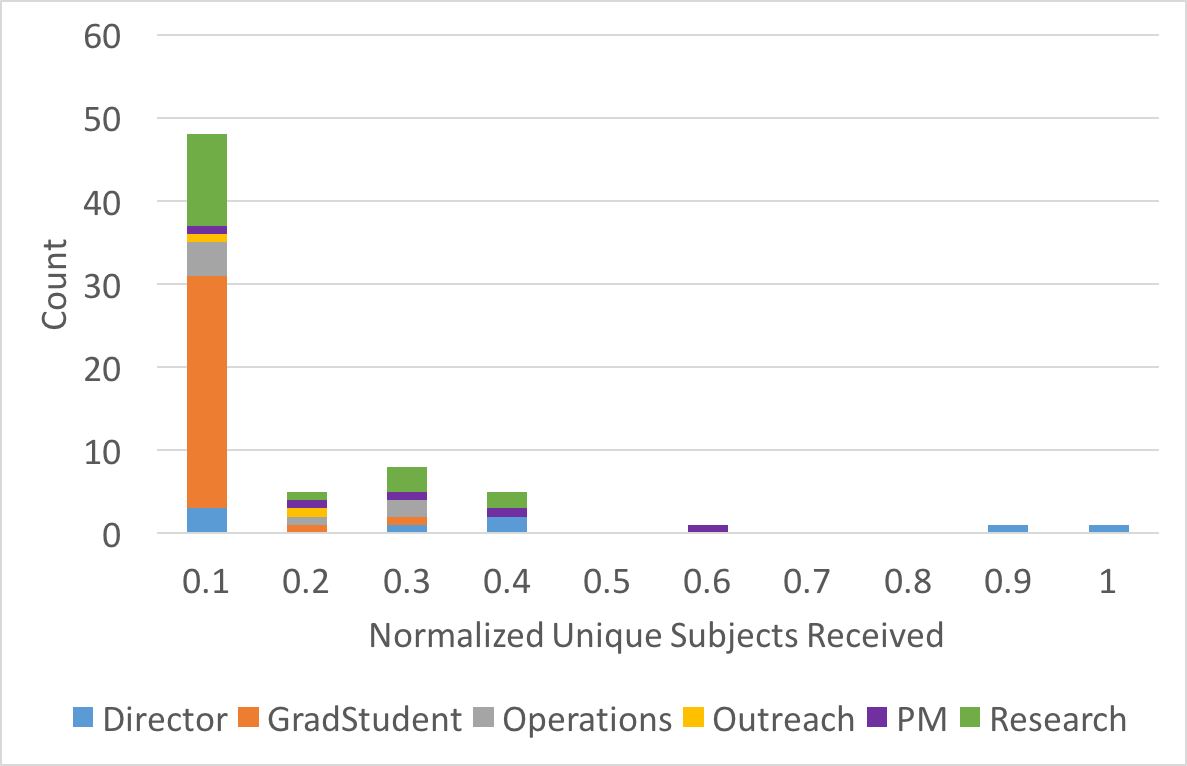
\includegraphics[width=\columnwidth,trim={1mm 17mm 1mm 2mm},clip]{Unique_subjects_rec_hist}
        \caption[Unique subjects received histogram]{Histogram of unique subjects received by job title.  The feature value for this plot has been normalized so that all values fall between 0 and 1.  Note that by using different thresholds, meaningful splits in the data can be made.  For example, all but two graduate students have a value less than $0.1$.}
        \label{fig:traffic_ex_hist}
\end{figure}

The second best traffic feature was the number of signed emails received.
Signed emails usually signal sensitive information.
Only certain groups within the center deal with this type of information, therefore it is understandable that this feature could help divide the subjects by title.
Finally, the third best traffic feature was the number of emails received as forwards.
Typically, those higher in the chain of command are forwarded emails where graduate students and lower-level employees are more likely to receive either replies or emails sent directly to them.
Notice that there are intuitive explanations behind all of the features selected by the ranker.


\subsection{Social Network Features}
\subsubsection{Social Network Representation}
In addition to tracking metadata statistics, features are also derived from modeling the emails as a social network.
A social network is composed of nodes, which represent people, and edges, which represent the emails between people.
For this analysis, two different graphs were generated for analysis.
In the full graph, an edge exists between any two individuals that exchanged at least one email.
Each edge was given a weight equal to the total number of emails exchanged between the two employees.
The edges are undirected for this analysis.
A second graph only produces the same weighted edge between two nodes but only if at least 10 emails were exchanged.
The purpose of this second graph is to filter out stray single-email relationships between coworkers that do not constitute meaningful communication.
The full graph including only the study volunteers is plotted in Figure~\ref{fig:social_net}.  Note that graduate students are found on the fringes of the network and are generally the least connected.  However, there is a clear core group of employees that communicate very frequently.


\begin{figure}[t]
    \centering
    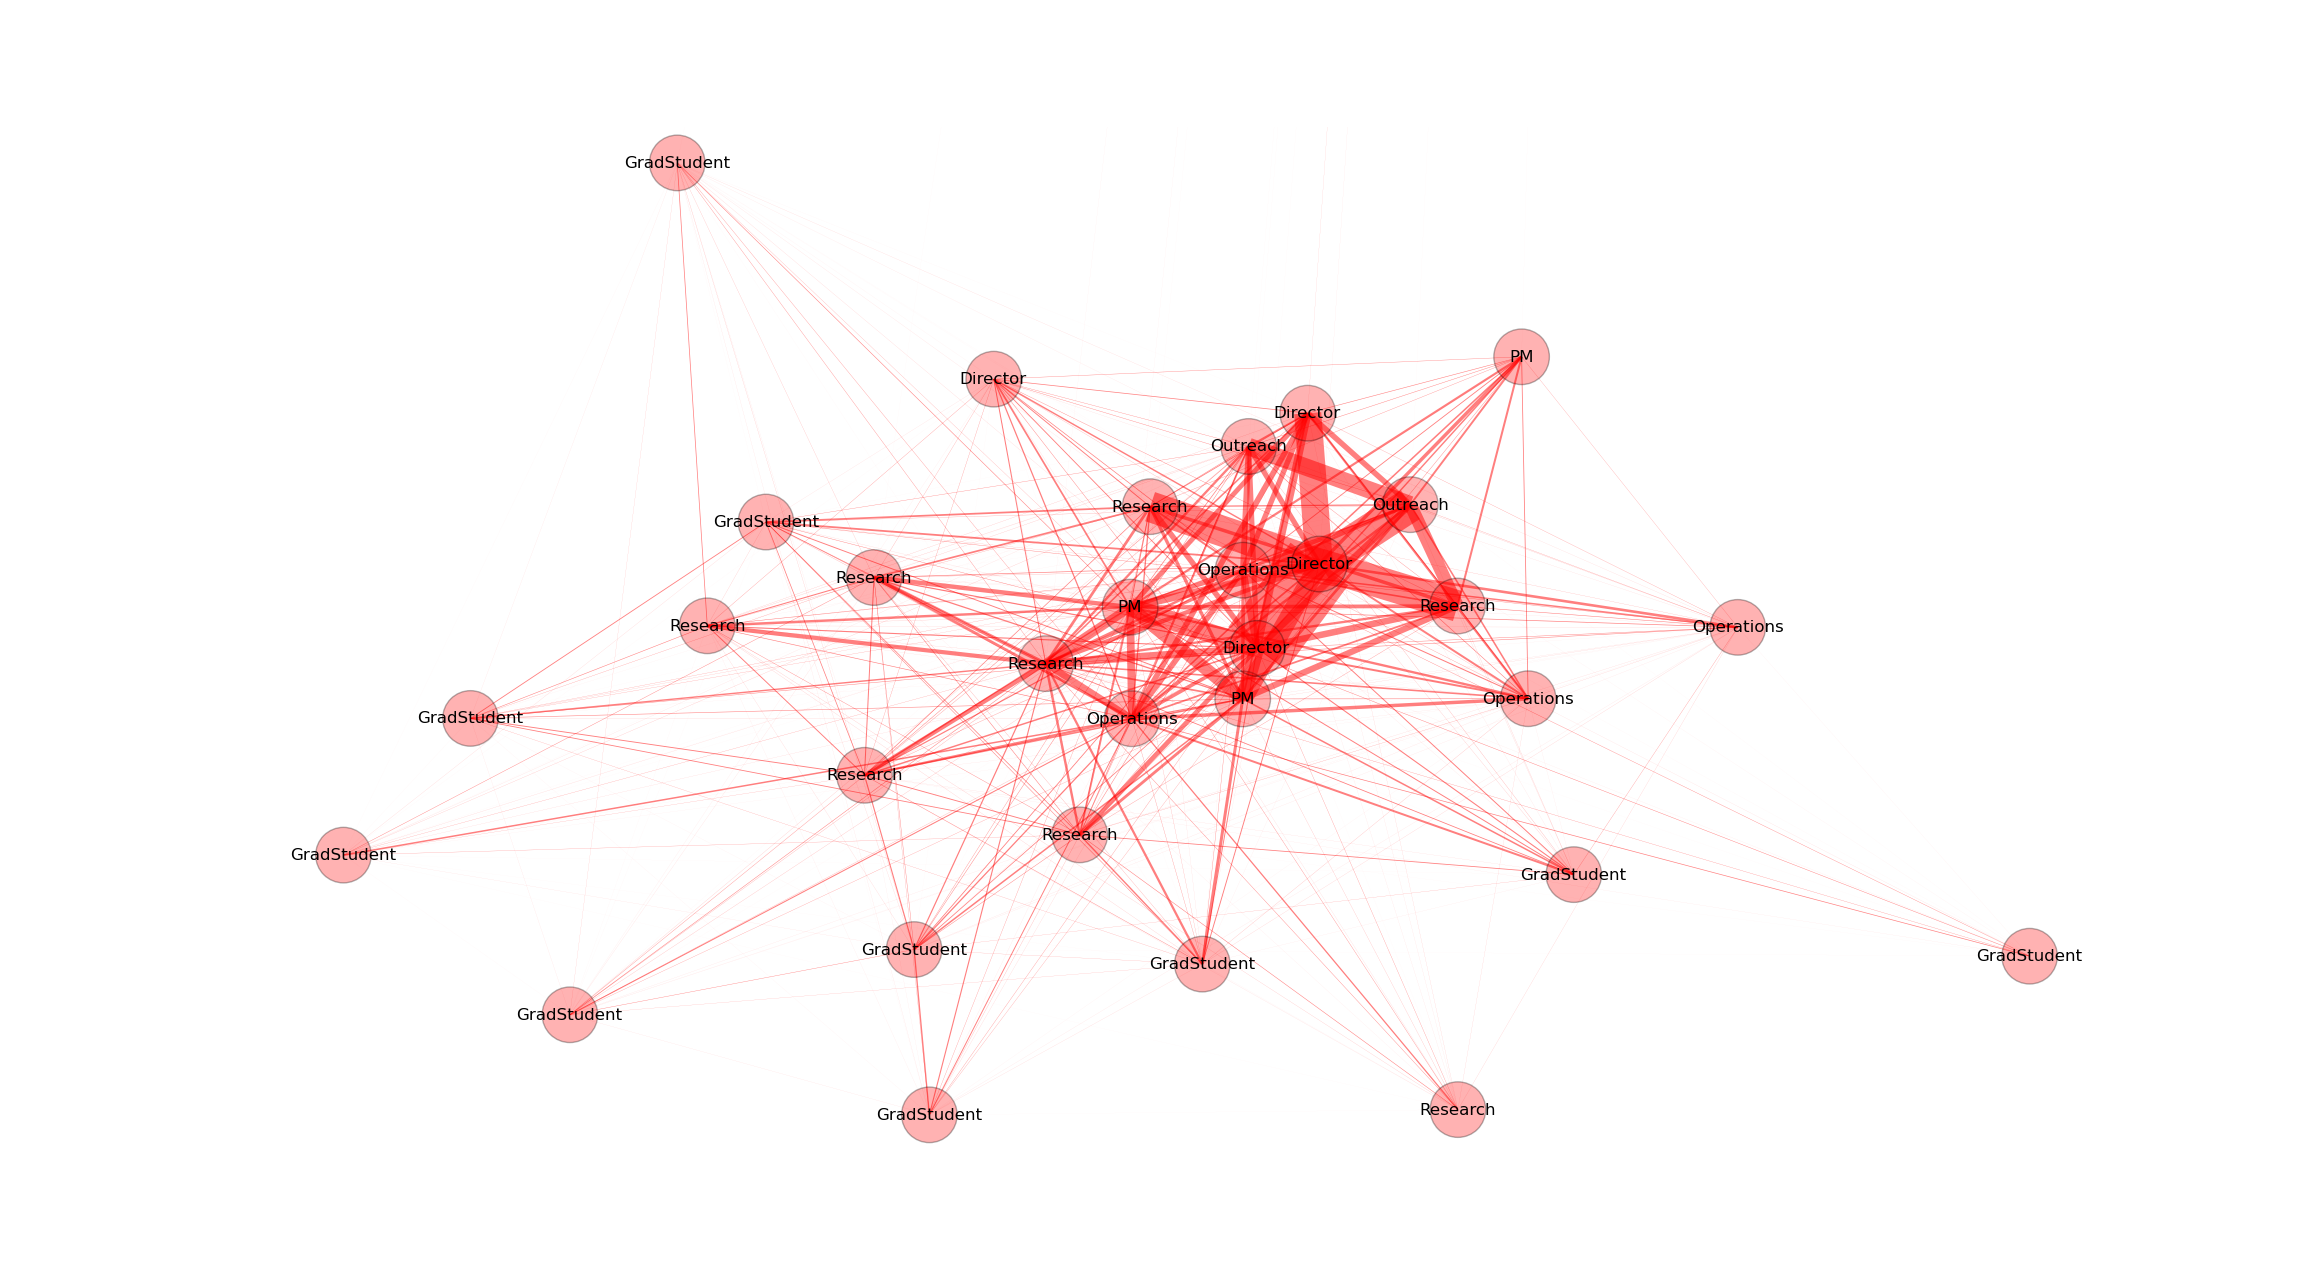
\includegraphics[width=\columnwidth,trim={4mm .5mm 0mm 5mm},clip]{HumeGraph2}
    \vspace{-17pt}
    \caption[The social network of the center]{A social graph representation of the center.  Nodes represent employees, and the thickness of the edges between nodes represent how many emails were exchanged.}
    \label{fig:social_net}
\end{figure}

Another representation of the full graph is shown as an adjacency matrix in Figure~\ref{fig:adj_matrix}.
Each of the two axes represent the employees of the center.
The color at each coordinate indicates how much communication existed between the two employees.
Some employees never exchanged any emails, while others exchanged many.

\begin{figure}[t]
    \centering
    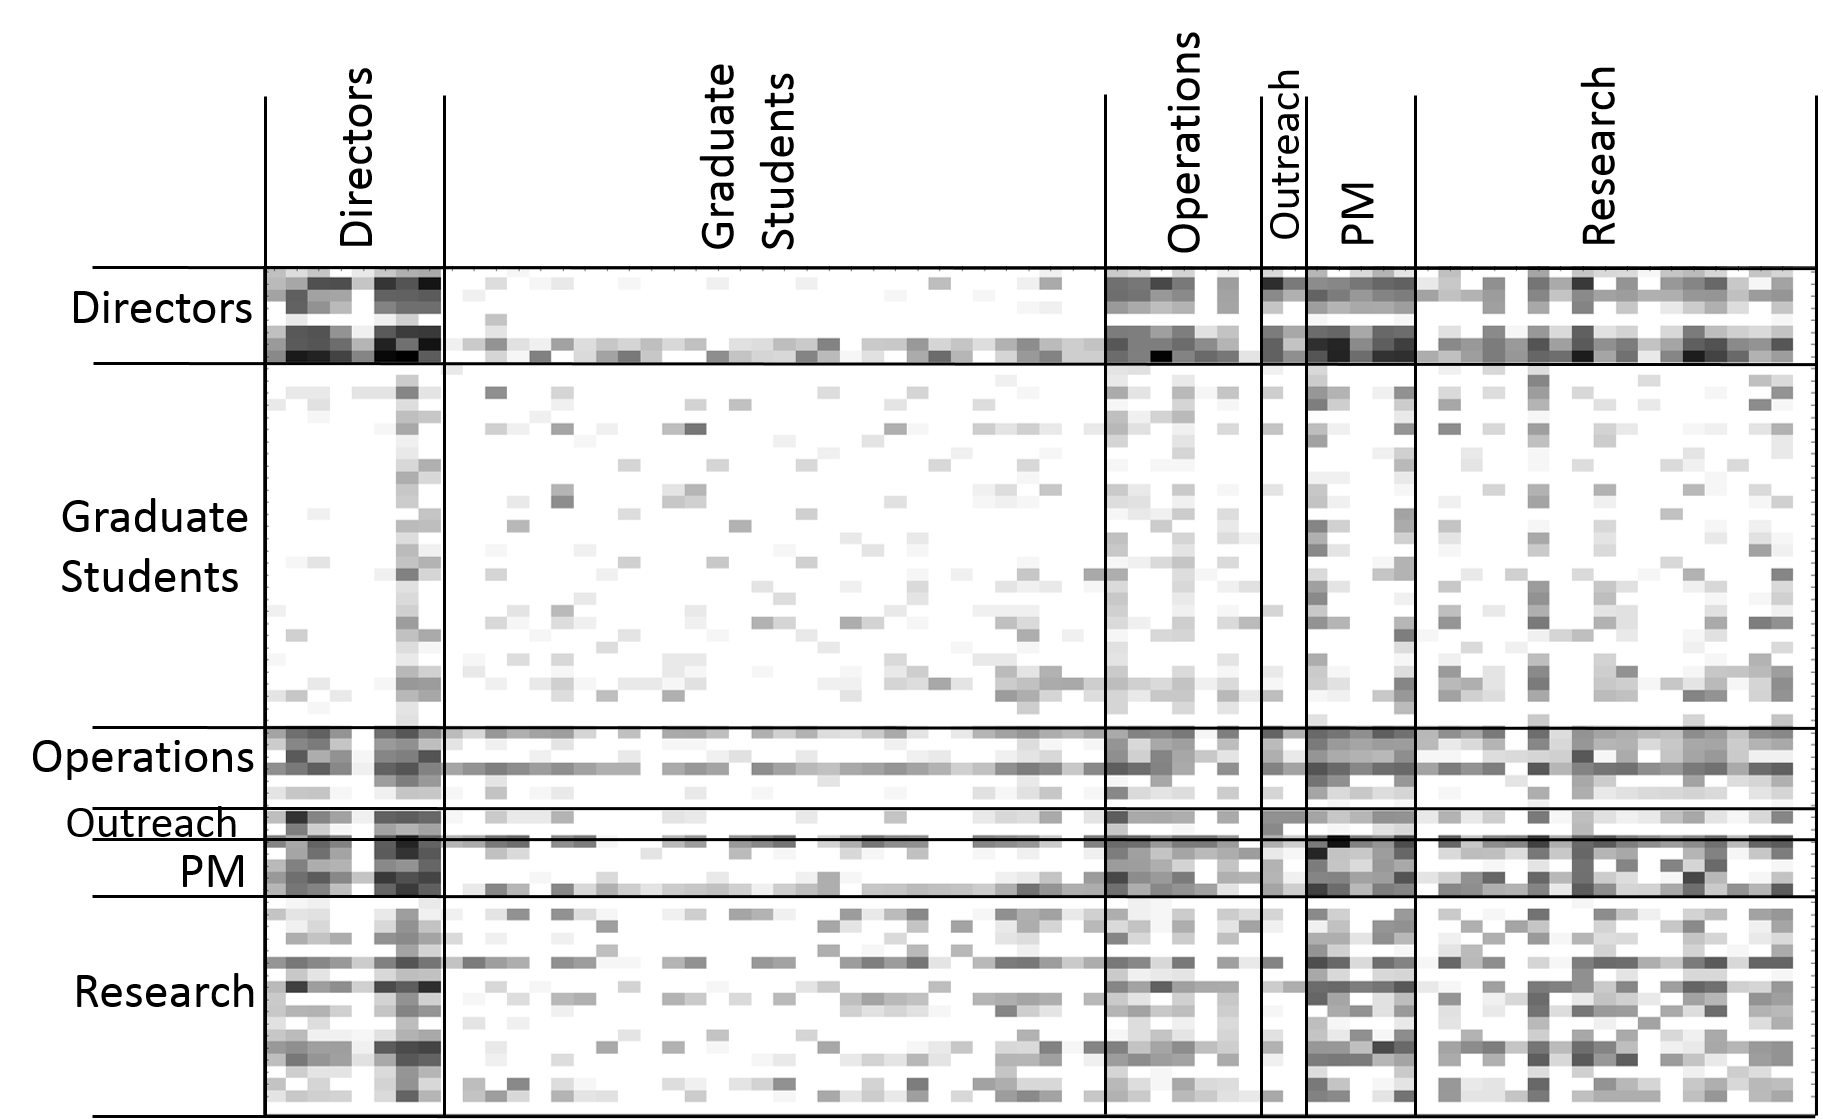
\includegraphics[width=\columnwidth,trim={4mm .5mm 0mm 5mm},clip]{adj_matrix}
    \vspace{-17pt}
    \caption[The dataset represented as an adjacency matrix]{The adjacency matrix representing the social connections of the center.  This graph is very well connected with just one component.  Nonetheless, there are many pairs of individuals who never exchanged a single email.}
    \label{fig:adj_matrix}
\end{figure}

Using this model, another suite of statistics can be calculated about the people in the graph.

\subsubsection{Degree Measures}
The degree of each node, from both the full and partial graph, was used as a feature.  
The degree of a node $i$ is simply the number of other edges connected to node $i$.
All graph features were calculated once for the full graph and again for the partial graph.
The average neighbor degree was calculated used as another feature.
The neighborhood of node $i$ is comprised of all nodes that are connected to $i$ via edges.
Therefore for node $i$, this metric averages the degree of each node in the neighborhood of $i$.
Mathematically, this is:
\begin{equation}
k_{\text{avg},i} = \frac{1}{|N(i)|}\sum_{j \in N(i)}k_j
\end{equation}
where $N(i)$ are the neighbors of node $i$ and $k_j$ is the degree of node $j$.
The distance between nodes were also used to generate some features.
In graph theory, distance is measured by the length of the path between two nodes.
Between node $i$ and any other node $j$ in graph $\mathcal{G}$, there exists a shortest path, $d(i,j)$.
The average shortest path between node $i$ and all other nodes in the graph, $d_avg,i$, was used as a metric for the learning algorithm.
That is,
\begin{equation}
d_{avg,i} = \frac{1}{n-1}\sum_{j \in \mathcal{V}, j\neq i}d(i,j)
\end{equation}
where $n$ is the number of nodes in graph $\mathcal{G}$ and $\mathcal{V}$ is the set of nodes in $\mathcal{G}$.
Similarly, the maximum shortest path length, or eccentricity, was used as a feature in the learning algorithm.
All of these measures can be interpreted to represent the centrality of a node.
If a node has many neighbors with large degrees or if it has very short maximum shortest paths it is probably representative of a person well-connected within the center.

\subsubsection{Cliques}
Some of the social features were based on existing graph theory concepts and algorithms.
For example, cliques.
If a subgraph of a graph $\mathcal{G}$ is maximally connected, that is all nodes are connected directly to each other, then this is called a maximal clique.
The number of cliques to which a node belongs was used as a feature.
The motivation behind using this metric is that it should mirror working groups within the center.
Therefore, the more groups an employee belongs to or communicates with, the more important they are assumed to be.

\subsubsection{Adapting Search Engine Algorithms}

The hubs and authorities of each node in both graphs were calculated.
The terms hubs and authorities come from the Hyperlink-Induced Topic Search (HITS algorithm) developed by~\cite{kleinberg_hubs_1999}.
This algorithm was originally designed to rate web pages, but has since been applied to social networks.
A node's authority is just that\textemdash{}a measure of its importance over other nodes.
A node's hub score is a measure of how well-connected it is to other nodes.

Another algorithm used to generate features was the pagerank algorithm, developed by Google \cite{page_pagerank_1999} also to rank webpages for search results.
The assumption is that the most important webpages will be linked to frequently by other pages.
Therefore, the ranking is determined by estimating the quality and quantity of links to a node.
Both of these algorithms were shown to predict expertise within an online social network in \cite{zhang_expertise_2007}.

\subsubsection{Clustering Metrics}
The triangle clustering coefficient, $C_3$ was also used as a metric.
Say there exists a node $i$ with neighbors $m$ and $n$.
This value, developed by~\cite{saramaki_generalizations_2007}, measures the probability that $m$ and $n$ are also connected.
This is calculated by comparing the number of triangles within the graph to the maximum number of possible triangles in the graph.  If node $i$ has degree $k_i$, there can be at most $\frac{k_i(k_i-1)}{2}$ triangles formed in this subgraph.  Recall that the social networks are weighted graphs.  The weights of the graph are incorporated to this metric by finding the geometric mean \cite{zhang_expertise_2007}.   Therefore, triangle clustering coefficient for node $i$, $C_{3,i}$, is:
\begin{equation}
C_{3,i} = \frac{2}{k_i(k_i-1)}\sum_{m,n}(\tilde{w}_{i,m}\tilde{w}_{m,n}\tilde{w}_{n,i})^\frac{1}{3}
\end{equation}

The edge weights in this calculation must be normalized compared to the maximum weight in the subgraph, i.e. $\tilde{w}_{i,m} = \frac{w_{i,m}}{max(w_{i,m})}$.

The square clustering coefficient is very similar and was also used in the algorithm.
This metric, developed by~\cite{lind_cycles_2005}, measures the probability that $m$ and $n$ are also neighbors to a fourth node, $p$.
This configuration would form a square.
To simplify the calculations, the graph for this metric is viewed without edge weights.
Therefore, the square clustering coefficient for node $i$, $C_{4,i}$, is the proportion of actual squares within a subgraph centered around node $i$ to the maximum number of possible squares in the same subgraph.
This is calculated as:
\begin{equation}
C_{4,i} = \frac{\sum_{m=1}^{k_i}\sum_{n=m+1}^{k_i}q_i(m,n)}{\sum_{m=1}^{k_i} \sum_{n=m+1}^{k_i}\left[a_i(m,n)+q_i(m,n) \right]}
\end{equation}

where $q_i(m,n)$ is the number of neighbors shared by $m$ and $n$, excluding $i$ and 
\begin{equation}
a_i(m,n) = (k_m-\eta_i(m,n))(k_n-\eta_i(m_n)) 
\end{equation}

where $\eta_i(m,n) = 1+q_i(m,n)+\theta_{mn}$.  
It is defined that $\theta_{mn}$ is an indicator function that takes on a value of 1 if $m$ and $n$ are neighbors and 0 otherwise.
In theory, the higher the clustering coefficient, the more connected the node is within its neighborhood.

\subsubsection{Centrality Measures}
The majority of the social-based features were variations on centrality measures.
First is closeness centrality.
Closeness centrality, $C(i)$ is the normalized inverse of the sum of shortest path distances from node $i$ to all other nodes in the graph \cite{freeman_centrality_1978}.  It is calculated as follows:
\begin{equation}
C(i) = \frac{n-1}{\sum_{j=1}^{n-1}d(i,j)}
\end{equation}

where $n$ is the number of nodes in graph $\mathcal{G}$ and $d(i,j)$ is the minimum shortest path distance between node $i$ and node $j$.

Next is betweenness centrality.
In a graph, there exists a shortest path between any node $s$ and any other node $t$.  Betweenness centrality of a node $i$, $C_B(i)$, is the percentage of all shortest paths in graph $\mathcal{G}$ that traverse node $i$ \cite{freeman_set_1977}.
It is calculated:
\begin{equation}
C_B(i) = \sum_{s,t\in \mathcal{V}}\frac{\sigma(s,t|i}{\sigma(s,t)}
\end{equation}

where $\mathcal{V}$ is the set of all nodes in $\mathcal{G}$, $\sigma(s,t)$ is the number of shortest paths between $s$ and $t$, and $\sigma(s,t|i)$ is the number of those paths that pass through $i$.
It is further defined that if $s=t$, then $\sigma(s,t)=1$ and if $i\in s,t$, then $\sigma(s,t|i) = 0$.

Degree centrality of a node $i$, $C_{d,i}$ is simply the percentage of nodes within the graph that are connected to node $i$~\cite{borgatti2011analyzing}:
\begin{equation}
C_{d,i} = \frac{k_i}{(n-1)}
\end{equation}

where $k_i$ is the degree of node $i$ and $n$ is the number of nodes in graph $\mathcal{G}$.

Current flow betweenness centrality, also known as information centrality, is measured for each node.
In general, metrics related to betweenness centrality differs from the previous centrality measures in that they consider all paths between nodes instead of exclusively shortest paths.
Current flow betweenness centrality in particular was modeled after how current flows in electrical networks~\cite{brandes2005centrality}.
In circuits, current is distributed over the possible paths; in this metric a similar approach is taken to determine the information content of each path between two nodes.
For a graph $\mathcal{G}$ where all nodes are reachable, it is possible to construct a matrix $B$ such that:
\begin{gather}
b_{ii} = 1 + \text{sum of weights of all edges connected to node } i \\
b_{ij} = 1- w_{ij}
\end{gather}

where $w_{ij}$ is the weight of the edge connecting nodes $i$ and $j$.
If $i$ and $j$ are not neighbors, $w_{ij}$ is defined to be $0$.
Denote $B^{-1} = C$.
From this matrix, the current flow betweenness centrality of node $i$, $I_i$, is calculated as:
\begin{equation}
I_i = \frac{n}{nc_{ii}+T-2R}
\end{equation}

where $n$ is the number of nodes in $\mathcal{G}$, $T$ is the sum of the diagonal elements, $T = \sum_{j=1}^nc_{jj}$, and $R$ is the sum of any row in $C$, $R = \sum_{j=1}^nc_{ij}$.
Note that because the matrix is symmetric, all rows of $C$ will have the same sum, therefore $R$ is not dependent on $i$~\cite{stephenson1989rethinking}.

This includes current flow closeness centrality, current flow betweenness centrality, communicability centrality, communicability betweenness centrality~\cite{estrada2008communicability}, and load centrality~\cite{newman2001scientific}.

All of these different graph statistics were used as inputs into the random forest algorithm to characterize each node's importance in the social graph.

\subsubsection{Most Useful Social Network Features}
The histogram of hub values in the full graph broken down by class is shown in Figure~\ref{fig:social_ex_hist}.

\begin{figure}[t]
    \centering
        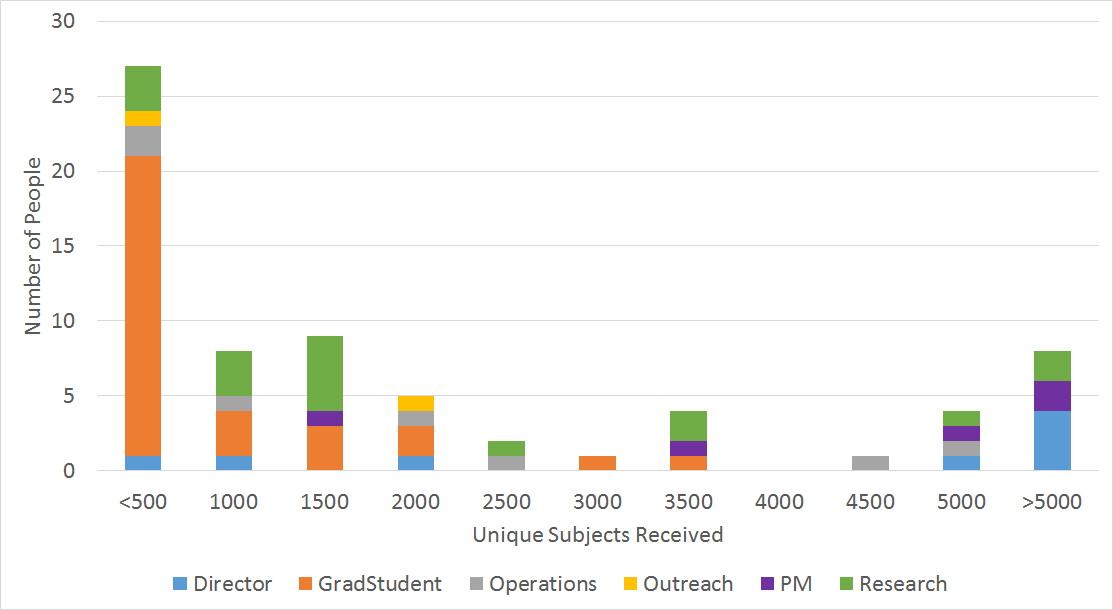
\includegraphics[width=\columnwidth,trim={.6mm 2mm 0.6mm 3mm},clip]{Hubs_hist}
        \vspace{-17pt}
        \caption[Full graph hubs histogram]{Histogram of hubs from social graph by job title.  Note that directors on average have the highest hub score and graduate students have the lowest.  In fact, three out of eight directors can be identified by filtering samples on full graph hubs values $>0.6$. }
        \label{fig:social_ex_hist}
\end{figure}
\chapter{Algorithm Design} \label{Algorithm}
\section{Tools}
\section{Model Selection}
Due to the large number of features and relatively low number of participants, a classification method was carefully chosen to avoid overfitting the data.
While tree based classifiers can be susceptible to overfitting, the random forest is robust to overfitting issues and was therefore chosen for this study.
The java-based software package Weka was used to generate the random forest based on the algorithm described in~\cite{Breiman2001}.

Random forests are an ensemble method of machine learning, comprised of many random trees.
A random tree is a machine learning algorithm that uses training data to learn a series of rules for classification.
These rules are constructed in a hierarchy that visually resembles a tree.
Each decision is based on what rule will maximize the information gained.
An example random tree with depth three is shown in Figure~\ref{fig:ex_tree}.

\begin{figure}[t]
    \centering
    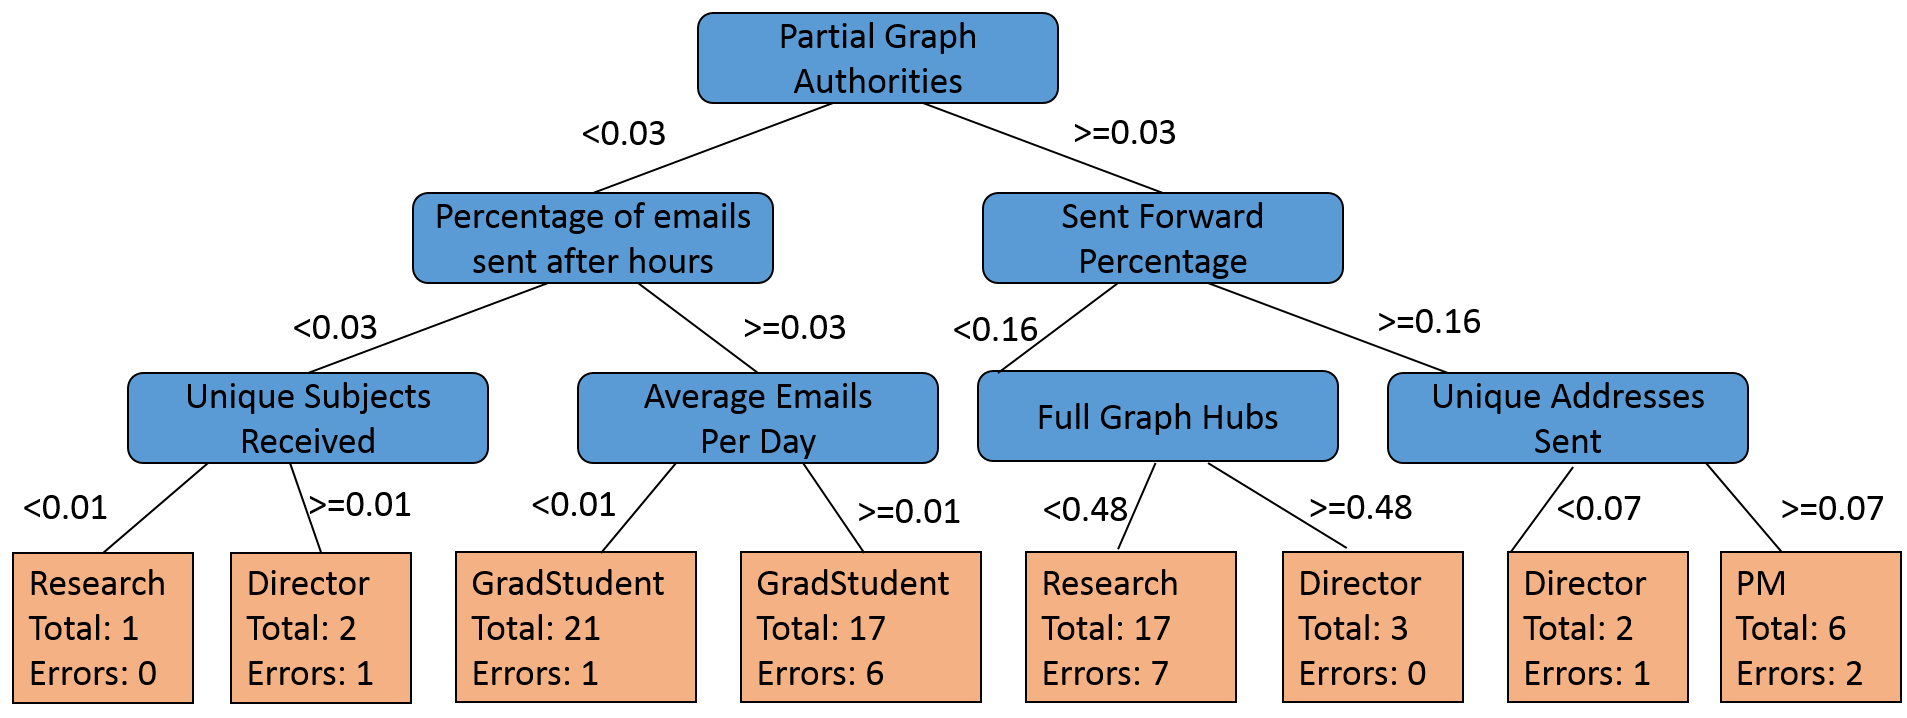
\includegraphics[width=\columnwidth,trim={0mm 2.5mm 0mm 2mm},clip]{3_level_tree}
    \vspace{-15pt}
    \caption[Example random tree]{Example random tree of depth 3 to demonstrate how a few rules can be used to find significant class divisions.}
    \label{fig:ex_tree}
\end{figure}

Random forests build deep random trees with slight random variations.
Individually, these random trees overfit the data.
However, these random trees are combined through a process of bootstrap aggregating, or bagging.
The number of trees was chosen to be 750 based empirical analysis.
The bagging process involves each random tree generating a new training data set by sampling observations from the input training set with replacement.
These subsamples are used to build the random trees.
For this analysis, each tree selects $\frac{2N}{3}$ samples to train the trees where $N$ is the number of data points in the overall training set.
Just as the samples were subsampled, so were the features.
Only this subset of features can be used as rules for that tree.
In this implementation, each tree used a subsample of 15 random features.

After all the trees are built, the test data is run through all the random trees in the forest.
Each tree outputs a prediction label for each data point, and the majority vote on each sample is the final predicted label.
This random forest model reduces the variance and increases the accuracy of the model compared to a single random tree.

\section{Feature Selection}
Random forests can be difficult to interpret because the ensemble method obscures which features are most meaningful.
An attribute analysis helps to better understand which features are better label predictors.
Since random trees use information gain to dictate splits, information gain was used as the evaluation criteria for the features.
Specifically, each attribute was evaluated by measuring the information gain with respect to the class.
Information gain is calculated as follows:
\begin{equation}
I(\text{Class}; \text{Attribute}) = H(\text{Class}) - H(\text{Class} | \text{Attribute})
\end{equation} \label{eq:info_gained}
where $I(\text{Class}; \text{Attribute})$ represents the mutual information between the class and the attribute, $H(Class)$ is the entropy of the class variable, and  $H(\text{Class} | \text{Attribute})$ represents the conditional entropy of the Class given the Attribute value.  

Mutual information represents how well knowledge of the attribute informs the prediction of the class.
In this model, both the attribute and the class are treated as random variables.
The entropy of a random variable is a measure of the uncertainty associated with it.
After this information gained value was calculated for each feature, they were ranked in order of most important to least.
Table~\ref{tab:ranked_feats} shows the top twenty features from this analysis and the features' corresponding information gain.

\begin{table}[t]
\caption{Top 20 features ranked by the information gain.}
\centering
\label{tab:ranked_feats}
\resizebox{0.6\columnwidth}{!}{%
\begin{tabular}{@{}lrr@{}}
\toprule
Feature                                      & Type         & Ranker \\ \midrule
Unique subjects received                     & Traffic      & 0.728  \\
Total signed emails received                 & Traffic      & 0.728  \\
Number of emails received as forwards        & Traffic      & 0.719  \\
Full graph hubs                              & Graph        & 0.589  \\
Partial graph communicability centrality     & Graph        & 0.554  \\
PG communicability betweenness centrality    & Graph        & 0.554  \\
Number of emails received as CC              & Traffic      & 0.507  \\
Percentage of emails received as forwards    & Traffic      & 0.503  \\
Partial graph degree centrality              & Graph        & 0.492  \\
Partial graph pagerank                       & Graph        & 0.492  \\
PG current flow closeness centrality         & Graph        & 0.492  \\
Average number of emails received per day    & Traffic      & 0.489  \\
Average total emails per day                 & Traffic      & 0.479  \\
Partial graph average shortest paths         & Graph        & 0.476  \\
Partial graph closeness centrality           & Graph        & 0.476  \\
Unique email addresses from signed emails    & Traffic      & 0.457  \\
Number of emails sent as CC                  & Traffic      & 0.43   \\
Number of emails received as replies         & Traffic      & 0.43   \\
Average emails sent per day                  & Traffic      & 0.404  \\ \bottomrule
\end{tabular}
}
\end{table}


\chapter{Performance Analysis} \label{Performance}
The results section first shows the algorithm's ability to correctly classify both the study's volunteers and the additional employees identified from the volunteers' emails.
The second part of the results section assumes perfect labeling of the employees and analyzes interactions between employees of different job titles.
The ultimate goal of this research was to determine what additional information can be gained by analyzing the organic organizational chart when compared with the official organizational chart.

\section{Classification Results}
Data was split by randomly assigning each email to either the training or testing set with equal probability.
Then, all of the metrics described in Section~\ref{Data} were calculated for both groups separately.
The training data was used as input to the random forest algorithm as described in Section~\ref{Algorithm}, and predictions were generated for the test data.
The number of correct and incorrect classifications for each class are shown below in Figure~\ref{fig:result_hist}.
Note that only two predictions were wrong: one person each in research and outreach were misclassified as graduate students.
It is important to note that both  misclassifications are for employees who did not provide their emails for the study.
Therefore, the classification accuracy for the study participants is 100\%, correctly classified inferred employees is 93.75\%, and the overall accuracy of this method using all features is 97.1\%.

\begin{figure}[t]
    \centering
    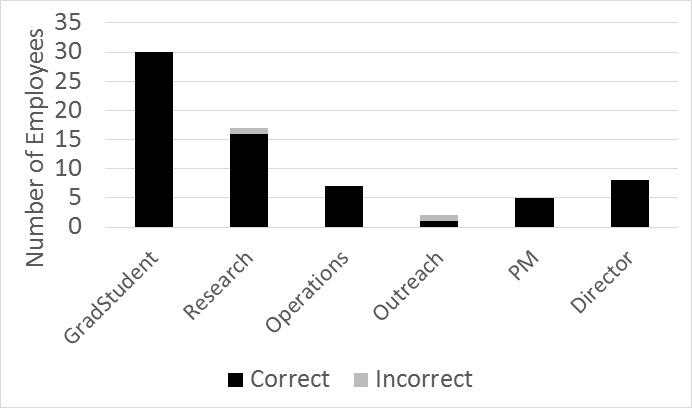
\includegraphics[width=\columnwidth,trim={1mm 2mm 1mm 3mm},clip]{Prediction_50_50_RF}
    \vspace{-20pt}
    \caption[Classification results]{The Random Forest algorithm was extremely accurate even for very uneven class sizes.  Note that all members of 4 classes were labelled perfectly.  There were only 2 errors out of 69 employees, both of which for employees who did not provide emails for the study.}
    \label{fig:result_hist}
\end{figure}

Note that this method relies on some assumptions.
One is that employees with the same title exhibit similar email behavior.
Overall, based on the success of the algorithm and the distributions of the histograms, this seems to prove true.
Another premise underlying this analysis is that peoples' email behaviors are consistent over time.
This seems to be true for the time range in this study.

To determine which features were necessary to the analysis, the algorithm was run several times with a subset of the features.
The first subset used only the top 20 features from Table~\ref{tab:ranked_feats}.
Using only these features resulted in 3 classification errors, or 95.6\% accuracy.
This is only one more error than was found using all 98 features.
For each subsequent run, the least useful feature according to the feature analysis was removed from the input to the system until only one feature remained.
A plot of this analysis is shown below in Figure \ref{fig:feat_analysis}.
Even using just the top thee features resulted in classification accuracy over 80\%.
Therefore, a very good classifier can be built using much fewer features if the features are selected properly.

\begin{figure}[t]
    \centering
        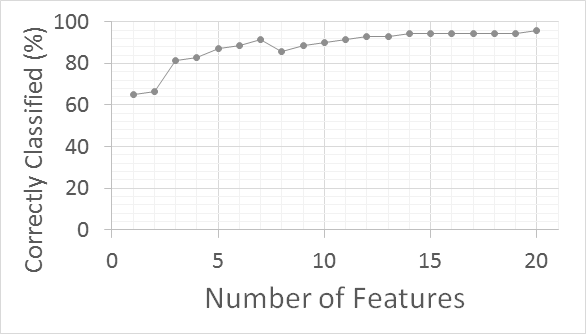
\includegraphics[width=.9\columnwidth,trim={1mm 6mm 1mm 3.5mm},clip]{FeatureAnalysis}
        \vspace{-7pt}
        \caption[Prediction accuracy compared to number of features]{Prediction accuracy compared to number of features used for analysis.  Note that the accuracy is still very high, 95.6\%, when only twenty features are used.  The outcome of using only the top twenty features produces three classification errors, only one more than using the full set of 98 features. }
        \label{fig:feat_analysis}
\end{figure}

\section{Leave-One Out Cross Validation}
So I tried LOOCV which gave, \ref{fig:loocv_conf_plot}.
\begin{figure}[t]
    \centering
        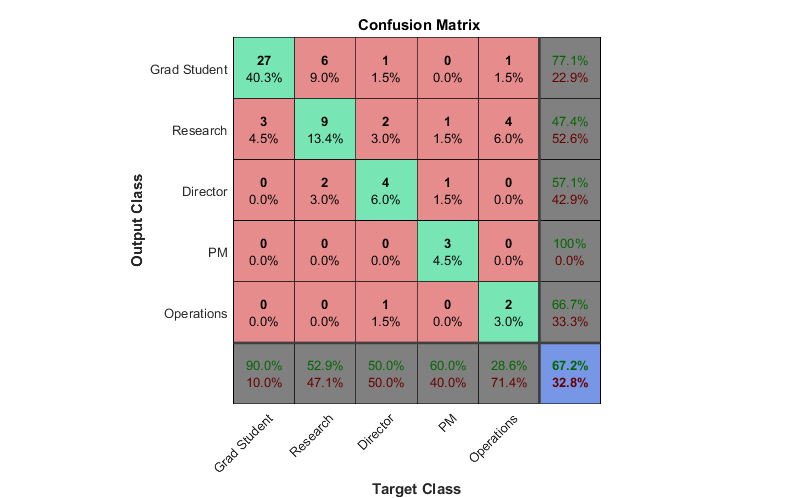
\includegraphics[width=.9\columnwidth,trim={1mm 4mm 1mm 3.5mm},clip]{confusion_plot}
        \vspace{-7pt}
        \caption[Leave one out cross validation results]{Prediction accuracy was higher for graduate students, who have more uniform behaviors and more training data.  However, for each category, the majority of the people classified were true members of that group, save for research.  Note that even for those classified as research, there were more true researchers than any other class.}
        \label{fig:loocv_conf_plot}
\end{figure}

\section{Hierarchy Analysis}
Most of the employees at the center are organized under a director and work with a program manager (unless for example they are a director or program manager).
To generate a metric of how well emails can be used to predict the center's organizational chart, the director and project manager for each applicable employee is predicted from the email metadata. 

The director of each employee is predicted by the algorithm to be the director that the employee communicated with most by email.
Only 57.58\% of the center's employees communicate most frequently with their official director.
This result points to a possible disconnect between the official organization chart and the organic relationships within the center.

To identify each employee's project manager ground truth is selected to be the project that primarily funds the employee.
This time, 72.73\% of graduate students and researchers communicate most frequently with their primary program manager.
The relation between employees to project managers appears to be stronger than that with directors.
Many of the errors in this classification are due to employees who work with multiple project managers.  

\chapter{Future Work} \label{FutureWork}
\section{Generalization}
\begin{itemize}
\item As discussed above, the accuracy of the leave-one-out cross-validation test was low because of the limited number of data points.  The confusion matrix in Figure \ref{fig:loocv_conf_plot} shows that about one third of the predictions were incorrect.  
\item These results can typically be improved by increasing the amount of training data. 
\item Performed experiment to gauge how the amount of training data affects the accuracy of the LOOCV test.  This is shown below in Figure  \ref{fig:loocv_generalization}.
\begin{figure}[t]
    \centering
        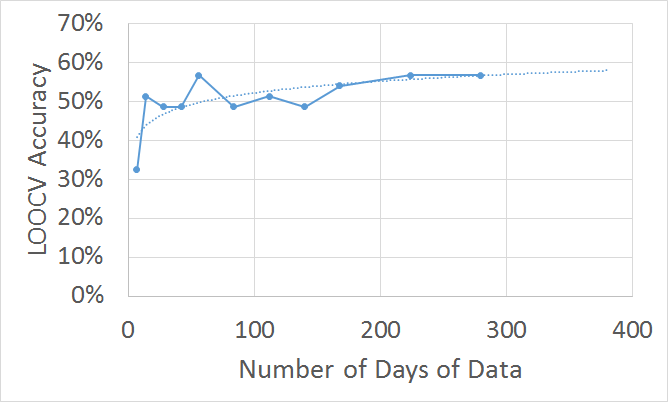
\includegraphics[width=.7\columnwidth,trim={1mm 2mm 1mm 3.5mm},clip]{generalization}
        \vspace{-7pt}
        \caption[Effects of more data on accuracy]{Effects of using more data for leave-one-out cross-validation.  [Still working on generating this, but I expect it to exponentially decrease.  From this data, I can fit a curve to the data that I do have to estimate how well the algorithm will perform with more data.]}
        \label{fig:loocv_generalization}
\end{figure}
\end{itemize}
\section{Deep Learning}
\begin{itemize}
\item Techniques such as random forests work well for small, low-dimensional data.  However, imagine if the size of the dataset were greatly increased to billions of people without labels.  In this case, a more sophisticated model would be necessary for successful classification.  This is required to accurately learn the complicated structure inherent to such large real-world datasets.
Suppose a representative sample of volunteers from the dataset self-identifies themselves.
This would produce a set of labeled training data, transforming the problem space to semi-supervised learning. 
\item Describe deep belief networks: A deep belief network is a generative graph with nodes that represent stochastic variables.
There are several layers of these nodes, some of which are visible and some are hidden.
Typically, the top two layers of nodes have undirected connections.
Therefore, these layers are actually Restricted Boltzman machines (RBMs).
The rest of the layers use directed edges, forming a Bayesian network.
For each node, there exists a probability of activation, $p(s_i=1)$, which is represented by the nonlinear sigmoid function applied to a weighted input from the layer above.
Specifically,
\begin{equation}
p(s_i=1) = \frac{1}{1+\exp \left(-b_i-\sum_j s_j w_{ij}\right)}
\end{equation}
where $j$ represents the ancestors of node $i$, $w_{ij}$ are the weights on the connections between $i$ and $j$, and $b_i$ is the bias associated with node $i$...
\item The challenge with very deep networks is that they are very difficult to train \cite{bengio_learning_2009}.
Unsupervised pre-training can improve the efficency of training deep belief networks, as first described in \cite{hinton_recognize_2007}.
In that work, Hinton describes a fast, greedy method to train these networks one layer at a time.  
\item 
Describe the process of unsupervised pre-training.
\item Testing on the MNIST dataset of handwritten digits, unsupervised pre-training is shown to improve classification results over only supervised training  \cite{erhan_why_2010}. 
Pre-training identifies a set of initial weights for the network that can ultimately lead to better classification results.  
An advantage of unsupervised pre-training is that, with small enough layers, it acts as a regularizer by decreasing variance and increasing the bias \cite{hinton_recognize_2007}.  
\item This labeled data can be used for backpropagation to fine-tune the network.
Describe the process backpropagation with the small set of labeled data.
\item In conjunction with greedy pre-training, backpropagation has been shown to improve both the optimization and generalization of a DBN. 
Hinton et al. showed that unsupervised pre-training followed by backpropagation of a DBN outperformed traditional feed forward neural networks on the MNIST dataset \cite{hinton_fast_2006}.
\item Analogous paper for comparison:\\
Much of the research in deep learning today is focused on image classification and analysis, such as the MNIST dataset.  However, DBNs have been applied to text analysis as well.  In \cite{ruangkanokmas_deep_2016}, a sophisticated version of a DBN was used to construct a sentiment classifier. The purpose of this research is to label online reviews as positive, negative, or neutral.  The difference between this method and other DBN approaches is that this work replaced some of the hidden layers of the network with a feature selection step.  Overall, this improves the training learning efficiency of the algorithm.  This method can classify sentiments more accurately and train more quickly than previous semi-supervised algorithms.
\end{itemize}



%If I had more data I could cluster but it would be rough.
%If I could label a few from each class, take 2 layers of neurons (greedily train).
%Use Boltzman's and backprop to get an awesome classifier!
%Write 3-4 pages on what more, higher-dimensional data + deep learning could improve.
%Show that I know how it works.



\chapter{Conclusions} \label{Conclusions}
This work presents a new dataset, approximately the size of Enron, that was collected from volunteers' emails with particular attention to protect participant privacy.
The new dataset includes accurate labels executed by researchers with knowledge of the center and its employees.
Statistics were calculated from this dataset, and were used with a random forest algorithm to automatically classify the center's employees.
Random Forests are shown to be powerful classifiers by predicting employee job titles with very high accuracy, even for employees for whom only secondhand data is available in the dataset.
Using only 3 features, employees are successfully classified higher than 80\% of the time and are classified over 95\% of the time when 20 features are used.
The email data was also used to show that emails could be used to predict an employee's primary program manager, but had a worse chance of being able to identify the director associated with the employee on the official organizational chart.
This work has shown that it is possible to generate important organizational information from using carefully processed email metadata without compromising the privacy of employees.
Future work will attempt to gain more insight into an organization's organic hierarchy and to apply these algorithms to other datasets to determine the general applicability of the results.




%%%%%%%%%%%%%%%%%
%
% Include an EPS figure with this command:
%   \epsffile{filename.eps}
%

%%%%%%%%%%%%%%%%
%
% Do tables like this:

% \begin{table}
% \caption{The Graduate School wants captions above the tables.}
%\begin{center}
% \begin{tabular}{ccc}
% x & 1 & 2 \\ \hline
% 1 & 1 & 2 \\
% 2 & 2 & 4 \\ \hline
% \end{tabular}
%\end{center}
% \end{table}

%%%%%%%%%%%%%%%%%%%%%%%%%%%%%%%%

\bibliographystyle{ieeetr}
\bibliography{bib}

% \appendix

% In LaTeX, each appendix is a "chapter"
% \chapter{Program Source}


\end{document}

